\documentclass{article}\usepackage[]{graphicx}\usepackage[]{color}
%% maxwidth is the original width if it is less than linewidth
%% otherwise use linewidth (to make sure the graphics do not exceed the margin)
\makeatletter
\def\maxwidth{ %
  \ifdim\Gin@nat@width>\linewidth
    \linewidth
  \else
    \Gin@nat@width
  \fi
}
\makeatother

\definecolor{fgcolor}{rgb}{0.345, 0.345, 0.345}
\newcommand{\hlnum}[1]{\textcolor[rgb]{0.686,0.059,0.569}{#1}}%
\newcommand{\hlstr}[1]{\textcolor[rgb]{0.192,0.494,0.8}{#1}}%
\newcommand{\hlcom}[1]{\textcolor[rgb]{0.678,0.584,0.686}{\textit{#1}}}%
\newcommand{\hlopt}[1]{\textcolor[rgb]{0,0,0}{#1}}%
\newcommand{\hlstd}[1]{\textcolor[rgb]{0.345,0.345,0.345}{#1}}%
\newcommand{\hlkwa}[1]{\textcolor[rgb]{0.161,0.373,0.58}{\textbf{#1}}}%
\newcommand{\hlkwb}[1]{\textcolor[rgb]{0.69,0.353,0.396}{#1}}%
\newcommand{\hlkwc}[1]{\textcolor[rgb]{0.333,0.667,0.333}{#1}}%
\newcommand{\hlkwd}[1]{\textcolor[rgb]{0.737,0.353,0.396}{\textbf{#1}}}%
\let\hlipl\hlkwb

\usepackage{framed}
\makeatletter
\newenvironment{kframe}{%
 \def\at@end@of@kframe{}%
 \ifinner\ifhmode%
  \def\at@end@of@kframe{\end{minipage}}%
  \begin{minipage}{\columnwidth}%
 \fi\fi%
 \def\FrameCommand##1{\hskip\@totalleftmargin \hskip-\fboxsep
 \colorbox{shadecolor}{##1}\hskip-\fboxsep
     % There is no \\@totalrightmargin, so:
     \hskip-\linewidth \hskip-\@totalleftmargin \hskip\columnwidth}%
 \MakeFramed {\advance\hsize-\width
   \@totalleftmargin\z@ \linewidth\hsize
   \@setminipage}}%
 {\par\unskip\endMakeFramed%
 \at@end@of@kframe}
\makeatother

\definecolor{shadecolor}{rgb}{.97, .97, .97}
\definecolor{messagecolor}{rgb}{0, 0, 0}
\definecolor{warningcolor}{rgb}{1, 0, 1}
\definecolor{errorcolor}{rgb}{1, 0, 0}
\newenvironment{knitrout}{}{} % an empty environment to be redefined in TeX

\usepackage{alltt}

% \usepackage[utf8]{inputenc}
\usepackage{amsmath}
\usepackage{fancyhdr}
\usepackage{array}
\usepackage{longtable}
\usepackage{graphicx}
\usepackage{color}
\usepackage[letterpaper, margin=1in]{geometry}
\usepackage{lscape}
\newcommand{\blandscape}{\begin{landscape}}
\newcommand{\elandscape}{\end{landscape}}
\usepackage{dcolumn}
\usepackage{bbm}
\usepackage{threeparttable}
\usepackage{booktabs}
\usepackage{expex}
\usepackage{pdflscape}
\usepackage{rotating, graphicx}
\usepackage{tabulary}
\usepackage{lscape}
\usepackage{makecell}
\usepackage{algorithm}
\usepackage{multirow}
\usepackage{colortbl}
\usepackage{longtable}
\usepackage{array}
\usepackage{multirow}
\usepackage{wrapfig}
\usepackage{float}
\usepackage{pdflscape}
\usepackage{tabu}
\usepackage{threeparttable}

\title{%
Homework 9\\
\large Applied Mutlivariate Analysis}
\date{November 1, 2018}
\author{Emorie Beck}
\IfFileExists{upquote.sty}{\usepackage{upquote}}{}
\begin{document}
\maketitle
% \SweaveOpts{concordance=TRUE}

\section{Workspace}
\subsection{Packages}



\begin{knitrout}
\definecolor{shadecolor}{rgb}{0.969, 0.969, 0.969}\color{fgcolor}\begin{kframe}
\begin{alltt}
\hlkwd{library}\hlstd{(car)}
\hlkwd{library}\hlstd{(knitr)}
\hlkwd{library}\hlstd{(psych)}
\hlkwd{library}\hlstd{(gridExtra)}
\hlkwd{library}\hlstd{(knitr)}
\hlkwd{library}\hlstd{(kableExtra)}
\hlkwd{library}\hlstd{(MASS)}
\hlkwd{library}\hlstd{(vegan)}
\hlkwd{library}\hlstd{(smacof)}
\hlkwd{library}\hlstd{(scatterplot3d)}
\hlkwd{library}\hlstd{(ape)}
\hlkwd{library}\hlstd{(ade4)}
\hlkwd{library}\hlstd{(ecodist)}
\hlkwd{library}\hlstd{(cluster)}
\hlkwd{library}\hlstd{(factoextra)}
\hlkwd{library}\hlstd{(ggdendro)}
\hlkwd{library}\hlstd{(lme4)}
\hlkwd{library}\hlstd{(plyr)}
\hlkwd{library}\hlstd{(tidyverse)}
\end{alltt}
\end{kframe}
\end{knitrout}



\subsection{data}
The file, Set\_7\_A.csv, contains data for 183 participants in a Pew Center Political Survey conducted in April 2017. Participants were asked their opinions about government spending using the following question stem:  

"If you were making up the budget for the federal government this year, would you increase spending, decrease spending or keep  spending the same for \_\_\_\_\_\_\_\_\_"?

The spending areas considered were:
\begin{itemize}
\item Scientific research
\item Militarydefense
\item Government assistance for the unemployed
\item Medicare
\item Environmental protection
\item Economic assistance to needy people around the world
\item Education
\end{itemize}

Responses were coded 1 = Decrease spending, 2 = Keep spending the same, and 3 = Increase spending.

\begin{knitrout}
\definecolor{shadecolor}{rgb}{0.969, 0.969, 0.969}\color{fgcolor}\begin{kframe}
\begin{alltt}
\hlstd{wd} \hlkwb{<-} \hlstr{"https://github.com/emoriebeck/homeworks/raw/master/multivariate/homeworks/homework9"}

\hlstd{datA} \hlkwb{<-} \hlkwd{sprintf}\hlstd{(}\hlstr{"%s/Set_7_A.csv"}\hlstd{, wd)} \hlopt \hlkwd{read.csv}\hlstd{(.,} \hlkwc{stringsAsFactors} \hlstd{= F)}
\hlstd{datB} \hlkwb{<-} \hlkwd{sprintf}\hlstd{(}\hlstr{"%s/Set_7_B.csv"}\hlstd{, wd)} \hlopt \hlkwd{read.csv}\hlstd{(.,} \hlkwc{stringsAsFactors} \hlstd{= F)}

\hlkwd{head}\hlstd{(datA)}
\end{alltt}
\begin{verbatim}
##   Spend_Science Spend_Military Spend_Unemployed Spend_Medicare
## 1             1              3                1              3
## 2             1              3                2              1
## 3             1              3                2              2
## 4             1              3                1              2
## 5             1              3                1              3
## 6             1              3                1              1
##   Spend_Environment Spend_World_Needy Spend_Education ID
## 1                 1                 1               3  1
## 2                 1                 1               1  2
## 3                 1                 1               2  3
## 4                 1                 1               2  4
## 5                 1                 1               2  5
## 6                 1                 1               2  6
\end{verbatim}
\begin{alltt}
\hlkwd{head}\hlstd{(datB)}
\end{alltt}
\begin{verbatim}
##   Age   Area_F               Trust_F             Gun_Control_F Sex_F
## 1  59    Rural                 Never Protect Right to Own Guns   Men
## 2  82    Rural Only Some of the Time Protect Right to Own Guns Women
## 3  40 Suburban Only Some of the Time Protect Right to Own Guns   Men
## 4  61    Rural Only Some of the Time Protect Right to Own Guns Women
## 5  70    Rural Only Some of the Time Protect Right to Own Guns   Men
## 6  63 Suburban Only Some of the Time Protect Right to Own Guns Women
##             Education_F Race_F     Income_F     Party_F        Ideology_F
## 1 Completed High School  White   30K to 40K  Republican      Conservative
## 2          Some College  White   50K to 75K  Republican      Conservative
## 3      Four-Year Degree  White   30K to 40K Independent Very Conservative
## 4          Some College  White 100K to 150K  Republican          Moderate
## 5         Post-Graduate  White   50K to 75K  Republican      Conservative
## 6      Four-Year Degree  White 100K to 150K  Republican          Moderate
##   ID
## 1  1
## 2  2
## 3  3
## 4  4
## 5  5
## 6  6
\end{verbatim}
\end{kframe}
\end{knitrout}

\section{Question 1}
First, use Ward’s procedure with Euclidean distance to determine how many clusters of respondents best describe this sample. Use the following procedures to arrive at the best choice:  

\subsection{Part A-D}
Run Ward’s procedure on a file that has been re-ordered using values for the military spending variable. Save the cluster memberships for a two-cluster solution. Repeat this procedure after re-ordering the file using values for the environmental protection variable. Repeat this procedure after re-ordering the file using values for the education variable. When you are done, you will have three new cluster membership variables, each from a Ward’s method applied to a different ordered version of the file. Create a cross-classification table for each pair of cluster membership variables. Are cases classified consistently regardless of how the data were ordered? 

Repeat this process, but for a three-cluster solution.

\begin{knitrout}
\definecolor{shadecolor}{rgb}{0.969, 0.969, 0.969}\color{fgcolor}\begin{kframe}
\begin{alltt}
\hlstd{dist_fun} \hlkwb{<-} \hlkwa{function}\hlstd{(}\hlkwc{dat}\hlstd{)\{}\hlkwd{dist}\hlstd{(dat} \hlopt \hlkwd{select}\hlstd{(}\hlopt{-}\hlstd{ID))\}}
\hlstd{cut_fun_w} \hlkwb{<-} \hlkwa{function}\hlstd{(}\hlkwc{dat}\hlstd{,} \hlkwc{C}\hlstd{,} \hlkwc{k}\hlstd{)\{dat}\hlopt{$}\hlstd{CW} \hlkwb{<-} \hlkwd{cutree}\hlstd{(C,} \hlkwc{k} \hlstd{= k); dat\}}
\hlstd{cut_fun_k} \hlkwb{<-} \hlkwa{function}\hlstd{(}\hlkwc{dat}\hlstd{,} \hlkwc{C}\hlstd{,} \hlkwc{k}\hlstd{)\{dat}\hlopt{$}\hlstd{CK} \hlkwb{<-} \hlstd{C}\hlopt{$}\hlstd{cluster; dat\}}

\hlstd{nested.models} \hlkwb{<-} \hlkwd{tribble}\hlstd{(}
  \hlopt{~}\hlstd{k,} \hlopt{~}\hlstd{order,} \hlopt{~}\hlstd{data,}
  \hlnum{2}\hlstd{,} \hlstr{"Spend_Military"}\hlstd{, datA} \hlopt \hlkwd{arrange}\hlstd{(Spend_Military),}
  \hlnum{3}\hlstd{,} \hlstr{"Spend_Military"}\hlstd{, datA} \hlopt \hlkwd{arrange}\hlstd{(Spend_Military),}
  \hlnum{4}\hlstd{,} \hlstr{"Spend_Military"}\hlstd{, datA} \hlopt \hlkwd{arrange}\hlstd{(Spend_Military),}
  \hlnum{5}\hlstd{,} \hlstr{"Spend_Military"}\hlstd{, datA} \hlopt \hlkwd{arrange}\hlstd{(Spend_Military),}
  \hlnum{2}\hlstd{,} \hlstr{"Spend_Environment"}\hlstd{, datA} \hlopt \hlkwd{arrange}\hlstd{(Spend_Environment),}
  \hlnum{3}\hlstd{,} \hlstr{"Spend_Environment"}\hlstd{, datA} \hlopt \hlkwd{arrange}\hlstd{(Spend_Environment),}
  \hlnum{4}\hlstd{,} \hlstr{"Spend_Environment"}\hlstd{, datA} \hlopt \hlkwd{arrange}\hlstd{(Spend_Environment),}
  \hlnum{5}\hlstd{,} \hlstr{"Spend_Environment"}\hlstd{, datA} \hlopt \hlkwd{arrange}\hlstd{(Spend_Environment),}
  \hlnum{2}\hlstd{,} \hlstr{"Spend_Education"}\hlstd{, datA} \hlopt \hlkwd{arrange}\hlstd{(Spend_Education),}
  \hlnum{3}\hlstd{,} \hlstr{"Spend_Education"}\hlstd{, datA} \hlopt \hlkwd{arrange}\hlstd{(Spend_Education),}
  \hlnum{4}\hlstd{,} \hlstr{"Spend_Education"}\hlstd{, datA} \hlopt \hlkwd{arrange}\hlstd{(Spend_Education),}
  \hlnum{5}\hlstd{,} \hlstr{"Spend_Education"}\hlstd{, datA} \hlopt \hlkwd{arrange}\hlstd{(Spend_Education)}
\hlstd{)} \hlopt
  \hlkwd{mutate}\hlstd{(}\hlkwc{D} \hlstd{=} \hlkwd{map}\hlstd{(data, dist_fun),}
         \hlkwc{C} \hlstd{=} \hlkwd{map}\hlstd{(D,} \hlopt{~}\hlkwd{hclust}\hlstd{(.,} \hlkwc{method} \hlstd{=} \hlstr{"ward.D2"}\hlstd{)),}
         \hlkwc{D} \hlstd{=} \hlkwd{pmap}\hlstd{(}\hlkwd{list}\hlstd{(data, C, k), cut_fun_w),}
         \hlkwc{K} \hlstd{=} \hlkwd{map2}\hlstd{(data, k, kmeans),}
         \hlkwc{D} \hlstd{=} \hlkwd{pmap}\hlstd{(}\hlkwd{list}\hlstd{(D, K, k), cut_fun_k))}

\hlstd{cross.class} \hlkwb{<-} \hlstd{nested.models} \hlopt \hlkwd{unnest}\hlstd{(D)} \hlopt
  \hlkwd{select}\hlstd{(k, order, CW, ID)} \hlopt
  \hlkwd{spread}\hlstd{(}\hlkwc{key} \hlstd{= order,} \hlkwc{value} \hlstd{= CW)} \hlopt
  \hlkwd{select}\hlstd{(}\hlopt{-}\hlstd{ID)} \hlopt
  \hlkwd{group_by}\hlstd{(k)} \hlopt
  \hlkwd{summarize}\hlstd{(}\hlkwc{`Edu-Env`} \hlstd{=} \hlkwd{list}\hlstd{(}\hlkwd{table}\hlstd{(Spend_Education, Spend_Environment)),}
            \hlkwc{`Edu-Mil`} \hlstd{=} \hlkwd{list}\hlstd{(}\hlkwd{table}\hlstd{(Spend_Education, Spend_Military)),}
            \hlkwc{`Env-Mil`} \hlstd{=} \hlkwd{list}\hlstd{(}\hlkwd{table}\hlstd{(Spend_Environment, Spend_Military)))}

\hlstd{(cross.class} \hlopt \hlkwd{filter}\hlstd{(k} \hlopt{==} \hlnum{2}\hlstd{))}\hlopt{$}\hlstd{`Edu-Env`[[}\hlnum{1}\hlstd{]]}
\end{alltt}
\begin{verbatim}
##                Spend_Environment
## Spend_Education   1   2
##               1  63   0
##               2   0 120
\end{verbatim}
\begin{alltt}
\hlstd{(cross.class} \hlopt \hlkwd{filter}\hlstd{(k} \hlopt{==} \hlnum{2}\hlstd{))}\hlopt{$}\hlstd{`Edu-Mil`[[}\hlnum{1}\hlstd{]]}
\end{alltt}
\begin{verbatim}
##                Spend_Military
## Spend_Education   1   2
##               1   0  63
##               2 120   0
\end{verbatim}
\begin{alltt}
\hlstd{(cross.class} \hlopt \hlkwd{filter}\hlstd{(k} \hlopt{==} \hlnum{2}\hlstd{))}\hlopt{$}\hlstd{`Env-Mil`[[}\hlnum{1}\hlstd{]]}
\end{alltt}
\begin{verbatim}
##                  Spend_Military
## Spend_Environment   1   2
##                 1   0  63
##                 2 120   0
\end{verbatim}
\begin{alltt}
\hlstd{(cross.class} \hlopt \hlkwd{filter}\hlstd{(k} \hlopt{==} \hlnum{3}\hlstd{))}\hlopt{$}\hlstd{`Edu-Env`[[}\hlnum{1}\hlstd{]]}
\end{alltt}
\begin{verbatim}
##                Spend_Environment
## Spend_Education  1  2  3
##               1 63  0  0
##               2  0  0 46
##               3  0 74  0
\end{verbatim}
\begin{alltt}
\hlstd{(cross.class} \hlopt \hlkwd{filter}\hlstd{(k} \hlopt{==} \hlnum{3}\hlstd{))}\hlopt{$}\hlstd{`Edu-Mil`[[}\hlnum{1}\hlstd{]]}
\end{alltt}
\begin{verbatim}
##                Spend_Military
## Spend_Education  1  2  3
##               1  0  0 63
##               2  0 46  0
##               3 74  0  0
\end{verbatim}
\begin{alltt}
\hlstd{(cross.class} \hlopt \hlkwd{filter}\hlstd{(k} \hlopt{==} \hlnum{3}\hlstd{))}\hlopt{$}\hlstd{`Env-Mil`[[}\hlnum{1}\hlstd{]]}
\end{alltt}
\begin{verbatim}
##                  Spend_Military
## Spend_Environment  1  2  3
##                 1  0  0 63
##                 2 74  0  0
##                 3  0 46  0
\end{verbatim}
\begin{alltt}
\hlstd{(cross.class} \hlopt \hlkwd{filter}\hlstd{(k} \hlopt{==} \hlnum{4}\hlstd{))}\hlopt{$}\hlstd{`Edu-Env`[[}\hlnum{1}\hlstd{]]}
\end{alltt}
\begin{verbatim}
##                Spend_Environment
## Spend_Education  1  2  3  4
##               1 29  0 34  0
##               2  0  0  0 46
##               3  0 32  0  0
##               4  0 42  0  0
\end{verbatim}
\begin{alltt}
\hlstd{(cross.class} \hlopt \hlkwd{filter}\hlstd{(k} \hlopt{==} \hlnum{4}\hlstd{))}\hlopt{$}\hlstd{`Edu-Mil`[[}\hlnum{1}\hlstd{]]}
\end{alltt}
\begin{verbatim}
##                Spend_Military
## Spend_Education  1  2  3  4
##               1  0  0 29 34
##               2  0 46  0  0
##               3 32  0  0  0
##               4 42  0  0  0
\end{verbatim}
\begin{alltt}
\hlstd{(cross.class} \hlopt \hlkwd{filter}\hlstd{(k} \hlopt{==} \hlnum{4}\hlstd{))}\hlopt{$}\hlstd{`Env-Mil`[[}\hlnum{1}\hlstd{]]}
\end{alltt}
\begin{verbatim}
##                  Spend_Military
## Spend_Environment  1  2  3  4
##                 1  0  0 29  0
##                 2 74  0  0  0
##                 3  0  0  0 34
##                 4  0 46  0  0
\end{verbatim}
\begin{alltt}
\hlstd{(cross.class} \hlopt \hlkwd{filter}\hlstd{(k} \hlopt{==} \hlnum{5}\hlstd{))}\hlopt{$}\hlstd{`Edu-Env`[[}\hlnum{1}\hlstd{]]}
\end{alltt}
\begin{verbatim}
##                Spend_Environment
## Spend_Education  1  2  3  4  5
##               1 29  0  0  0  0
##               2  0  0 34  0  0
##               3  0  0  0  0 46
##               4  0 22  0 10  0
##               5  0  0  0 42  0
\end{verbatim}
\begin{alltt}
\hlstd{(cross.class} \hlopt \hlkwd{filter}\hlstd{(k} \hlopt{==} \hlnum{5}\hlstd{))}\hlopt{$}\hlstd{`Edu-Mil`[[}\hlnum{1}\hlstd{]]}
\end{alltt}
\begin{verbatim}
##                Spend_Military
## Spend_Education  1  2  3  4  5
##               1  0  0  0 29  0
##               2  0  0  0  0 34
##               3  0  0 46  0  0
##               4 17 15  0  0  0
##               5  5 37  0  0  0
\end{verbatim}
\begin{alltt}
\hlstd{(cross.class} \hlopt \hlkwd{filter}\hlstd{(k} \hlopt{==} \hlnum{5}\hlstd{))}\hlopt{$}\hlstd{`Env-Mil`[[}\hlnum{1}\hlstd{]]}
\end{alltt}
\begin{verbatim}
##                  Spend_Military
## Spend_Environment  1  2  3  4  5
##                 1  0  0  0 29  0
##                 2  9 13  0  0  0
##                 3  0  0  0  0 34
##                 4 13 39  0  0  0
##                 5  0  0 46  0  0
\end{verbatim}
\end{kframe}
\end{knitrout}

The data are relatively inconsistently classified depending on the ordering. With larger k, the data seem to be classified more consistently. 

\subsection{Part E}
(e) Of these solutions, which one provides the highest number of clusters while being completely immune to the ordering of the variables?  

The highest number of clusters that are aimmune to the ordering is 3 clusters.

\begin{knitrout}
\definecolor{shadecolor}{rgb}{0.969, 0.969, 0.969}\color{fgcolor}\begin{kframe}
\begin{alltt}
\hlstd{(cross.class} \hlopt \hlkwd{filter}\hlstd{(k} \hlopt{==} \hlnum{3}\hlstd{))}\hlopt{$}\hlstd{`Edu-Env`[[}\hlnum{1}\hlstd{]]}
\end{alltt}
\begin{verbatim}
##                Spend_Environment
## Spend_Education  1  2  3
##               1 63  0  0
##               2  0  0 46
##               3  0 74  0
\end{verbatim}
\begin{alltt}
\hlstd{(cross.class} \hlopt \hlkwd{filter}\hlstd{(k} \hlopt{==} \hlnum{3}\hlstd{))}\hlopt{$}\hlstd{`Edu-Mil`[[}\hlnum{1}\hlstd{]]}
\end{alltt}
\begin{verbatim}
##                Spend_Military
## Spend_Education  1  2  3
##               1  0  0 63
##               2  0 46  0
##               3 74  0  0
\end{verbatim}
\begin{alltt}
\hlstd{(cross.class} \hlopt \hlkwd{filter}\hlstd{(k} \hlopt{==} \hlnum{3}\hlstd{))}\hlopt{$}\hlstd{`Env-Mil`[[}\hlnum{1}\hlstd{]]}
\end{alltt}
\begin{verbatim}
##                  Spend_Military
## Spend_Environment  1  2  3
##                 1  0  0 63
##                 2 74  0  0
##                 3  0 46  0
\end{verbatim}
\end{kframe}
\end{knitrout}

\section{Question 2}
For the chosen number of clusters from Question 1, create a bar graph of the cluster means for each of the spending variables (include 95\% confidence intervals). Based on these graphs, provide a description of each cluster’s spending attitude profile.

\begin{knitrout}
\definecolor{shadecolor}{rgb}{0.969, 0.969, 0.969}\color{fgcolor}\begin{kframe}
\begin{alltt}
\hlstd{nested.models} \hlopt \hlkwd{filter}\hlstd{(k} \hlopt{==} \hlnum{3} \hlopt{&} \hlstd{order} \hlopt{==} \hlstr{"Spend_Military"}\hlstd{)} \hlopt
  \hlkwd{unnest}\hlstd{(D)} \hlopt
  \hlkwd{gather}\hlstd{(}\hlkwc{key} \hlstd{= cat,} \hlkwc{value} \hlstd{= value,} \hlkwd{contains}\hlstd{(}\hlstr{"Spend"}\hlstd{))} \hlopt
  \hlstd{Rmisc}\hlopt{::}\hlkwd{summarySE}\hlstd{(.,} \hlkwc{measurevar} \hlstd{=} \hlstr{"value"}\hlstd{,} \hlkwc{groupvars} \hlstd{=} \hlkwd{c}\hlstd{(}\hlstr{"CW"}\hlstd{,} \hlstr{"cat"}\hlstd{))} \hlopt
  \hlkwd{ggplot}\hlstd{(}\hlkwd{aes}\hlstd{(}\hlkwc{x} \hlstd{= cat,} \hlkwc{y} \hlstd{= value,} \hlkwc{fill} \hlstd{=} \hlkwd{factor}\hlstd{(CW)))} \hlopt{+}
    \hlkwd{scale_fill_manual}\hlstd{(}\hlkwc{values} \hlstd{= RColorBrewer}\hlopt{::}\hlkwd{brewer.pal}\hlstd{(}\hlnum{9}\hlstd{,} \hlstr{"Greens"}\hlstd{)[}\hlkwd{c}\hlstd{(}\hlnum{1}\hlstd{,}\hlnum{4}\hlstd{,}\hlnum{7}\hlstd{)])} \hlopt{+}
    \hlkwd{geom_bar}\hlstd{(}\hlkwc{stat} \hlstd{=} \hlstr{"identity"}\hlstd{,} \hlkwc{position} \hlstd{=} \hlstr{"dodge"}\hlstd{,} \hlkwc{color} \hlstd{=} \hlstr{"black"}\hlstd{)} \hlopt{+}
    \hlkwd{geom_errorbar}\hlstd{(}\hlkwd{aes}\hlstd{(}\hlkwc{ymin} \hlstd{= value} \hlopt{-} \hlstd{ci,} \hlkwc{ymax} \hlstd{= value} \hlopt{+} \hlstd{ci),}
                  \hlkwc{position} \hlstd{=} \hlkwd{position_dodge}\hlstd{(}\hlnum{.9}\hlstd{),} \hlkwc{width} \hlstd{=} \hlnum{.1}\hlstd{)} \hlopt{+}
    \hlkwd{labs}\hlstd{(}\hlkwc{x} \hlstd{=} \hlkwa{NULL}\hlstd{,} \hlkwc{y} \hlstd{=} \hlstr{"Mean Rating"}\hlstd{,} \hlkwc{fill} \hlstd{=} \hlstr{"Cluster"}\hlstd{)} \hlopt{+}
    \hlkwd{coord_flip}\hlstd{()} \hlopt{+}
    \hlkwd{theme_classic}\hlstd{()} \hlopt{+}
    \hlkwd{theme}\hlstd{(}\hlkwc{legend.position} \hlstd{=} \hlstr{"bottom"}\hlstd{)}
\end{alltt}
\end{kframe}
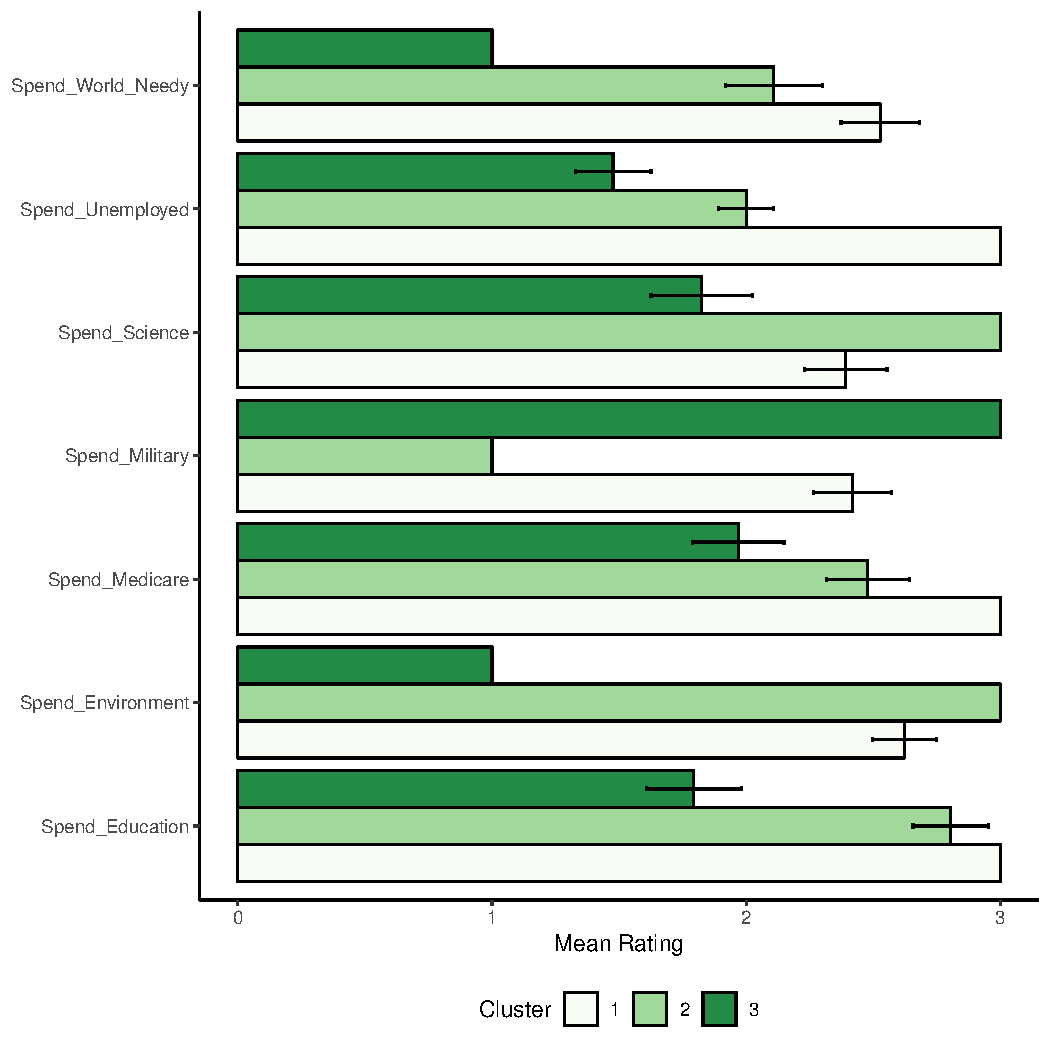
\includegraphics[width=\maxwidth]{figure/unnamed-chunk-6-1} 

\end{knitrout}

\section{Question 3}
Using K-means clustering, create a plot of the within-cluster sums of squares for cluster solutions up to 10. Does the number of clusters from this plot suggest the same number of clusters identified by Ward’s procedure?

\begin{knitrout}
\definecolor{shadecolor}{rgb}{0.969, 0.969, 0.969}\color{fgcolor}\begin{kframe}
\begin{alltt}
\hlstd{wssplot} \hlkwb{<-} \hlkwa{function}\hlstd{(}\hlkwc{data}\hlstd{,}\hlkwc{nc}\hlstd{=}\hlnum{15}\hlstd{,}\hlkwc{seed}\hlstd{=}\hlnum{1234}\hlstd{) \{}
  \hlstd{wss} \hlkwb{<-} \hlstd{(}\hlkwd{nrow}\hlstd{(data}\hlopt{-}\hlnum{1}\hlstd{))}\hlopt{*}\hlkwd{sum}\hlstd{(}\hlkwd{apply}\hlstd{(data,}\hlnum{2}\hlstd{,var))}
  \hlkwa{for} \hlstd{(i} \hlkwa{in} \hlnum{2}\hlopt{:}\hlstd{nc) \{}
    \hlkwd{set.seed}\hlstd{(seed)}
    \hlstd{wss[i]} \hlkwb{<-} \hlkwd{sum}\hlstd{(}\hlkwd{kmeans}\hlstd{(data,}\hlkwc{centers}\hlstd{=i)}\hlopt{$}\hlstd{withinss)}
  \hlstd{\}}
  \hlstd{plot_data} \hlkwb{<-} \hlkwd{cbind}\hlstd{(wss,}\hlkwd{seq}\hlstd{(}\hlnum{1}\hlstd{,nc,}\hlnum{1}\hlstd{))}
  \hlstd{plot_data} \hlkwb{<-} \hlkwd{as.data.frame}\hlstd{(plot_data)}
  \hlkwd{names}\hlstd{(plot_data)} \hlkwb{<-} \hlkwd{c}\hlstd{(}\hlstr{"wss"}\hlstd{,}\hlstr{"nc"}\hlstd{)}
  \hlkwd{ggplot}\hlstd{(plot_data,} \hlkwd{aes}\hlstd{(}\hlkwc{x}\hlstd{=nc,}\hlkwc{y}\hlstd{=wss))} \hlopt{+}
    \hlkwd{geom_point}\hlstd{(}\hlkwc{shape}\hlstd{=}\hlnum{19}\hlstd{,}\hlkwc{size}\hlstd{=}\hlnum{3}\hlstd{)} \hlopt{+}
    \hlkwd{geom_line}\hlstd{()} \hlopt{+}
    \hlkwd{scale_x_continuous}\hlstd{(}\hlkwc{breaks}\hlstd{=}\hlkwd{c}\hlstd{(}\hlkwd{seq}\hlstd{(}\hlnum{1}\hlstd{,nc,}\hlnum{1}\hlstd{)))} \hlopt{+}
    \hlkwd{xlab}\hlstd{(}\hlstr{"Number of Clusters"}\hlstd{)} \hlopt{+}
    \hlkwd{ylab}\hlstd{(}\hlstr{"Within-Cluster Sum of Squares"}\hlstd{)} \hlopt{+}
    \hlkwd{theme_classic}\hlstd{()} \hlopt{+}
  \hlkwd{ggtitle}\hlstd{(}\hlstr{"Within-Cluster Sums of Squares by Number of Clusters"}\hlstd{)}
\hlstd{\}}
\hlkwd{wssplot}\hlstd{(datA[,}\hlnum{1}\hlopt{:}\hlnum{7}\hlstd{],}\hlkwc{nc}\hlstd{=}\hlnum{10}\hlstd{)}
\end{alltt}
\end{kframe}
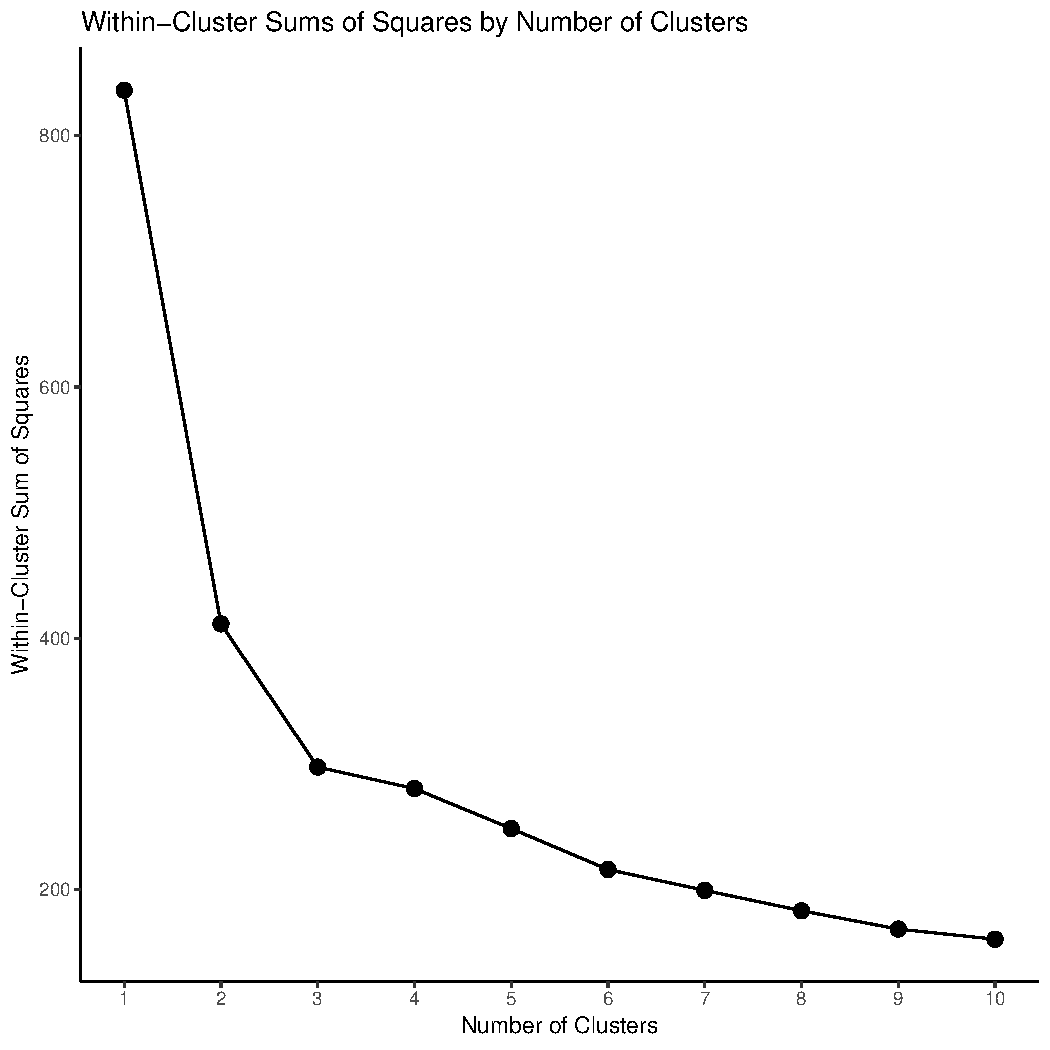
\includegraphics[width=\maxwidth]{figure/unnamed-chunk-7-1} 

\end{knitrout}

\section{Question 4}
For the chosen number of clusters from Question 1, conduct a K-means clustering of the data. Provide a cross-classification table for the Ward’s and K-means procedures. Do the two procedures identify the same clusters?

\begin{knitrout}
\definecolor{shadecolor}{rgb}{0.969, 0.969, 0.969}\color{fgcolor}\begin{kframe}
\begin{alltt}
\hlkwd{table}\hlstd{((nested.models} \hlopt \hlkwd{filter}\hlstd{(k} \hlopt{==} \hlnum{3}\hlstd{))}\hlopt{$}\hlstd{D[[}\hlnum{1}\hlstd{]]} \hlopt \hlkwd{select}\hlstd{(CW, CK))}
\end{alltt}
\begin{verbatim}
##    CK
## CW   1  2  3
##   1 37 21 16
##   2  2 40  4
##   3 22  0 41
\end{verbatim}
\end{kframe}
\end{knitrout}

The two procedures appear to identify slightly different clusters. 

\section{Question 5}
5. The file, Set\_7\_B.csv, contains additional information about these respondents. Use this file to better define the nature of the clusters identified in Question 4. The variables included in Set\_7\_B are age, home area (rural, urban, suburban), level of trust in the government, gun control attitude, sex, highest level of education, race, annual income, political party affiliation, and political ideology. Using these variables, what are the defining features of each cluster? Focus on those variables that do the best job of distinguishing the groups.

\begin{knitrout}
\definecolor{shadecolor}{rgb}{0.969, 0.969, 0.969}\color{fgcolor}\begin{kframe}
\begin{alltt}
\hlstd{(nested.models} \hlopt \hlkwd{filter}\hlstd{(k} \hlopt{==} \hlnum{3}\hlstd{))}\hlopt{$}\hlstd{D[[}\hlnum{1}\hlstd{]]} \hlopt \hlkwd{full_join}\hlstd{(datB)} \hlopt
  \hlkwd{select}\hlstd{(}\hlopt{-}\hlstd{(Spend_Science}\hlopt{:}\hlstd{Spend_Education))} \hlopt
  \hlkwd{group_by}\hlstd{(CW)} \hlopt \hlkwd{mutate}\hlstd{(}\hlkwc{N} \hlstd{=} \hlkwd{n}\hlstd{())} \hlopt
  \hlkwd{gather}\hlstd{(}\hlkwc{key} \hlstd{= category,} \hlkwc{value} \hlstd{= value,} \hlopt{-}\hlstd{ID,} \hlopt{-}\hlstd{CW,} \hlopt{-}\hlstd{CK,} \hlopt{-}\hlstd{Age,} \hlopt{-}\hlstd{N)} \hlopt
  \hlkwd{group_by}\hlstd{(CW, category, value)} \hlopt
  \hlkwd{summarize}\hlstd{(}\hlkwc{n} \hlstd{=} \hlkwd{n}\hlstd{()}\hlopt{/}\hlstd{N[}\hlnum{1}\hlstd{])} \hlopt
  \hlkwd{spread}\hlstd{(}\hlkwc{key} \hlstd{= CW,} \hlkwc{value} \hlstd{= n)}
\end{alltt}
\begin{verbatim}
## # A tibble: 42 x 5
## # Groups:   category [9]
##    category    value                           `1`     `2`    `3`
##    <chr>       <chr>                         <dbl>   <dbl>  <dbl>
##  1 Area_F      Rural                        0.176   0.174  0.270 
##  2 Area_F      Suburban                     0.473   0.283  0.460 
##  3 Area_F      Urban                        0.351   0.543  0.270 
##  4 Education_F Completed High School        0.297   0.0870 0.206 
##  5 Education_F Did Not Complete High School 0.0270 NA      0.0476
##  6 Education_F Four-Year Degree             0.216   0.348  0.238 
##  7 Education_F Post-Graduate                0.135   0.239  0.206 
##  8 Education_F Some College                 0.189   0.174  0.159 
##  9 Education_F Some Post-Graduate           0.0270 NA      0.0317
## 10 Education_F Two-Year Degree              0.108   0.152  0.111 
## # ... with 32 more rows
\end{verbatim}
\end{kframe}
\end{knitrout}

Cluster 1 appears to be moderate to liberal Independents and Democrats who are more suburban, support gun control, and contain a higher proportion of women and African Americans.\\
Cluster 2 appears to be moderate to liberal Independents and Democrats who are more ubran and support gun control.\\
Cluster 3 appears to be conservative Republicans who opposed gun control and are disproportionately white and male.

\begin{knitrout}
\definecolor{shadecolor}{rgb}{0.969, 0.969, 0.969}\color{fgcolor}\begin{kframe}
\begin{alltt}
\hlstd{(nested.models} \hlopt \hlkwd{filter}\hlstd{(k} \hlopt{==} \hlnum{3}\hlstd{))}\hlopt{$}\hlstd{D[[}\hlnum{1}\hlstd{]]} \hlopt \hlkwd{full_join}\hlstd{(datB)} \hlopt
  \hlkwd{select}\hlstd{(}\hlopt{-}\hlstd{(Spend_Science}\hlopt{:}\hlstd{Spend_Education))} \hlopt
  \hlkwd{group_by}\hlstd{(CK)} \hlopt \hlkwd{mutate}\hlstd{(}\hlkwc{N} \hlstd{=} \hlkwd{n}\hlstd{())} \hlopt
  \hlkwd{gather}\hlstd{(}\hlkwc{key} \hlstd{= category,} \hlkwc{value} \hlstd{= value,} \hlopt{-}\hlstd{ID,} \hlopt{-}\hlstd{CW,} \hlopt{-}\hlstd{CK,} \hlopt{-}\hlstd{Age,} \hlopt{-}\hlstd{N)} \hlopt
  \hlkwd{group_by}\hlstd{(CK, category, value)} \hlopt
  \hlkwd{summarize}\hlstd{(}\hlkwc{n} \hlstd{=} \hlkwd{n}\hlstd{()}\hlopt{/}\hlstd{N[}\hlnum{1}\hlstd{])} \hlopt
  \hlkwd{spread}\hlstd{(}\hlkwc{key} \hlstd{= CK,} \hlkwc{value} \hlstd{= n)}
\end{alltt}
\begin{verbatim}
## # A tibble: 42 x 5
## # Groups:   category [9]
##    category    value                           `1`     `2`    `3`
##    <chr>       <chr>                         <dbl>   <dbl>  <dbl>
##  1 Area_F      Rural                        0.246   0.180  0.197 
##  2 Area_F      Suburban                     0.410   0.393  0.459 
##  3 Area_F      Urban                        0.344   0.426  0.344 
##  4 Education_F Completed High School        0.262   0.213  0.164 
##  5 Education_F Did Not Complete High School 0.0164 NA      0.0656
##  6 Education_F Four-Year Degree             0.197   0.295  0.279 
##  7 Education_F Post-Graduate                0.164   0.197  0.197 
##  8 Education_F Some College                 0.213   0.164  0.148 
##  9 Education_F Some Post-Graduate           0.0164  0.0164 0.0328
## 10 Education_F Two-Year Degree              0.131   0.115  0.115 
## # ... with 32 more rows
\end{verbatim}
\end{kframe}
\end{knitrout}

Cluster 1 appears to be white and African American conservative to moderate Republicans and Independents who are split on gun control and slightly more rural than other clusters. \\
Cluster 2 appears to be predominantly white (and disproportionately male) conservative to moderate Republicans and Independents who oppose gun control\\
Cluster 3 appears to be white urban and suburban Democrats and Independents who support gun control.

\end{document}
